\documentclass[accentcolor=tud1a,colorbacktitle,inverttitle,landscape,german,presentation,t]{tudbeamer}
\usepackage{ngerman}

\begin{document}

\title[Fabelhafte Benner Boys]{Die Fabelhaften Benner Boys pr"asentieren
stolz das TUD-Corporate-Design f"ur beamer-\LaTeX}
\subtitle{Johannes Werner\\Clemens v. Loewenich\\tuddesign@pro-kevin.de}

\author[J. Werner et al.]{Johannes Werner and Clemens von Loewenich}
\institute[IFP TUD]{Institut f"ur Festk"orperphysik, TU Darmstadt}

\logo{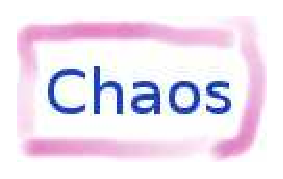
\includegraphics{TUDbeamer-logo}}
% \logo{\color{tudtextaccent}\large IFP}

\date{\today}

\begin{titleframe}
\end{titleframe}

\section{Einleitung}
	
	\subsection{Dokumentation}
		\begin{frame}
		  \frametitle{Optionen der \textbf{tudbeamer} Klasse}
			Die \textbf{tudbeamer} Klasse setzt auf
			\textbf{latex-beamer} Klasse auf. Neben deren
			Optionen gibt es zus"atzlich:
		  \begin{itemize}
			\item \textbf{accentcolor=$<$color$>$}
			\item \textbf{colorbacktitle}
			\item \textbf{colorback}
			\item \textbf{invertitle}
			\item \textbf{inverttitlerule}
			\item \textbf{blackrule}
			\item \textbf{tudmathserif}
		  \end{itemize}
			Die Optionen sind analog zur \textbf{tudreport} Klasse, bis auf \textbf{colorback}. 
			Diese Option hinterlegt die Titel aller Folien au"ser dem auf der Titelfolie.\\
			\vfill
			Ist die Akzentfarbe zu hell werden z.B. die Marken von
			Aufz"ahlungen in Schwarz gesetzt. Die verwendete
			Farbe ist "uber den Farbnamen \alert{\bf tudtextaccent}
			verwendbar.\\
			\vfill
			\textbf{tudmathserif} stellt den Mathe-Modus auf Serifenschriftart um
		\end{frame}

		\begin{frame}
		  \frametitle{Titleseite}
			F"ur die Titelseite gibt es eine Eigene Umgebung, die
			die richtigen beamertemplates setzt und
			\textbf{\textbackslash titlepage} ausf"uhrt.\\
			\vfill
			\textbf{\textbackslash begin$\{$titleframe$\}$\\
				\quad Inhalt der Titelseite\\
			        \textbackslash end$\{$titleframe$\}$}
			\vfill
			Erzeugt die Titelseite mit entsprechendem Inhalt, der
			am oberen Rand ausgerichtet wird.

		\end{frame}


\section{Erster Teil}

	\begin{frame}[t]
		\frametitle{Frametitle dieser Seite, ist zwar etwas lang,
		macht aber nix}
		Allgemeines bla-bla\dots Einleitung\dots und so weiter\\
		was auch immer hier zu sagen w"are\dots\\
		ach ja: das hier ist ein frame mit Argument [t]
	\end{frame}

\section{Zweiter Teil}

	\subsection{Unterpunkt}
		
		\begin{frame}[b]
		  \frametitle{kurzer Frametitle}
		\transdissolve[duration=0.5]
			Was wir schon immer mal in einer Pr"asentation ausprobieren wollten,
			aber uns nie so wirklich getraut haben. Ich werde das jetzt einfach
			mal so mit Beamertex setzen und hoffe, dass ich alles halbwegs
			hinbekomme\\

			Frame mit Argument [b]

		\end{frame}

	\subsection{Noch'n Unterpunkt}

		\begin{frame}[c]
		\transdissolve[duration=0.5]
			Was auch immer\dots

			Die Standardeinstellung ist leider [c] (centered), man
			kann aber was sinnvolles (also [t]) als Klassenoption angeben
			\begin{equation*}
				\frac{hijklmno}{HIJKLMNO}12345\alpha \beta
			\end{equation*}
		\end{frame}

\section{N"achster Teil}
	
	\begin{frame}
		{\bf Mit "Uberschrift}

		Ohne Unterpunkte\\

		Das "`Papier"' ist "ubrigens so gro"s:\\
		\the\paperheight ~ x~ \the\paperwidth
	\end{frame}

	\begin{frame}
		Hier ist jetzt also die Pr"asentation \emph{fast}
		zu ende\dots
		
		Es folgen noch zwei Folien mit Aufz"ahlungen.
	\end{frame}

	\begin{frame}
		\begin{itemize}
			\item Ich denke,
			\item das war's wohl
			\item mit diesem Test
		\end{itemize}
	\end{frame}

	\begin{frame}
		\begin{itemize}
			\item Ich denke,
			\item das war's wohl
			\item mit dieser Pr"asentation
		\end{itemize}
	\end{frame}

\end{document}

